\chapter{Focus Group} \label{chapter:focus-group}
As the user tests have shown, terminology is a major usability issue. Participants have been exposed to entirely new concepts they were not familiar with before. Errors that have been made during the sessions were often related to a misunderstanding of what a feature does. How things are phrased influences a user’s comprehension of a system, her mental model, heavily. As described in the related work section earlier Git’s conceptual model is flawed in certain ways, which is also reflected in the terminology. In order to avoid adopting these flaws for the content authoring tool, some Git concepts will be revised, reconsidered or combined in new ways. Therefore, new names need to be found for these concepts that reflect their purpose and help the user form an accurate mental model of the system.
%write how this was also about identifying what the difficult terms are -> more focus on discovery and getting insights than on generating new ideas

\section{Objectives}
First and foremost the focus group is intended to provide a better understanding of the user’s thought process. Which terms are hard to understand or even misleading? Can they derive a function’s purpose based on its name? Since the participants were already exposed to the terms and corresponding features they will be able to provide feedback based on their own experience. Besides gaining insights the focus group also aims at producing suggestions for improvements. How can terms be rephrased to allow an easier understanding?

\section{Procedure}
In the beginning the participants will get an overview of the agenda and a short introduction. The first phase consists of an open discussion among the participants. This should take no longer than 15 minutes. During this time the participants are going to talk about their difficulties when using the prototype in special regards to the naming of the functionality. In case the discussion steers off into a different direction the group moderator will try to focus the discussion on the naming again by asking specific questions.

In the second phase the participants are expected to come up with alternatives to the current names. During the user tests it became clear that most participants did not really understand what version control is and why they have to perform certain steps. For the focus group a more informed understanding of version control will be helpful so that the participants can reflect on why they struggled. Therefore, a short introduction to version control is given by the moderator. Afterwards the participants will be asked to imagine alternatives for the most problematic terms, which have been determined through a survey and the previous usability study. First, participants will generate ideas by themselves and write them down on paper. Afterwards the whole group will discuss those ideas and the pros and cons of the proposed solutions.

\section{Results}

\subsection{Pre-session survey}
In a short survey the participants were asked about how well they had understood different version control concepts based on their names. The table below lists the ones that were perceived to be most difficult to understand. The scale reached from 1 to 5, 1 reflecting a hard to understand term/concept and 5 an easy one.  

\begin{table}[h!]
\begin{tabular}{|r|l|}
\hline
\rowcolor[HTML]{EFEFEF} 
\multicolumn{1}{|l|}{\cellcolor[HTML]{EFEFEF}{\bf Score (mean)}} & {\bf Term}            \\ \hline
3.0                                                              & Pull Request          \\ \hline
3.4                                                              & Create (Pull Request) \\ \hline
3.4                                                              & Branch                \\ \hline
3.6                                                              & Merge (Pull Request)  \\ \hline
3.6                                                              & Reviewer              \\ \hline
\end{tabular}
\centering
\caption{Least understood version control concepts}
\label{table:concept-ratings}
\end{table}


\subsection{First Phase}
The first phase, the open discussion, showed that still a lot of confusion prevailed among the participants regarding the most common version control concepts. It is hard to say whether this is because of the names used for these concepts or because the concepts are inherently hard to understand. Branch and pull request, for example, seemed to be most problematic, but they are also conceptually the most complex. One of the participants even thought they are more or less the exact same thing. Another one mentioned, she could not tell the difference between the three concepts of unsaved changes, history and pull requests and had no idea in which order to use them. To conclude, one could say, that none of the participants (except for one) had formed an accurate mental model of the system, which is not surprising, given that they have only used it once and were not introduced to it before.

The participants agreed that it is easier to understand the concepts once they are explained first, but they also stated that freelancers likely will not have this luxury. One positive aspect that was highlighted is that the illustrations in the prototype helped form a more accurate comprehension of certain version control concepts (Figure 1). History, as one of the few concepts, seemed to be clear to most people. This also reflects the 4.0 average score in the pre-session survey. Something that is peculiar, is that the term unsaved changes fared well during the survey (4.2), but seemed to pose conceptual problems to some participants.

\begin{figure}[h!]
 \centering
 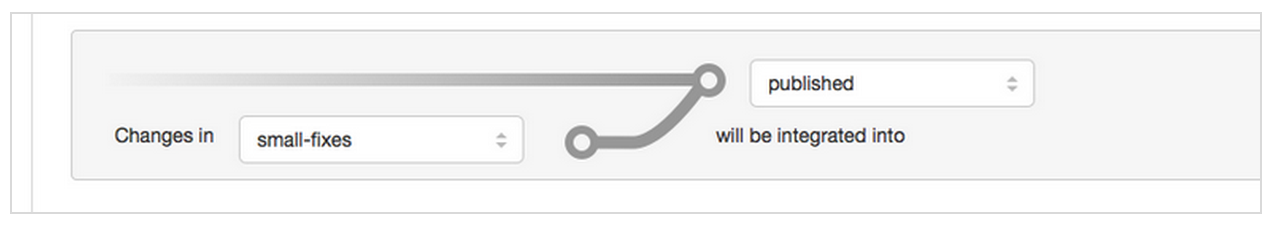
\includegraphics[width=\textwidth]{branch-visualization}
 \caption{Illustration that visualizes what happens when two branches are merged}
 \label{fig:branch-visualization}
\end{figure}

\subsection{Second Phase}
At the beginning of the second phase the moderator gave a short introduction to version control and the most important concepts. This was done to provide the participants with a solid understanding of version control and its concepts, thus making it easier for them to come up with alternative names. The brainstorming proved to be more difficult than expected, but yielded a handful of alternative terms for each concept that had been deemed hard to comprehend earlier. What made it difficult to find different names for some concepts was the large domain they have to work for. For example, a translator creates a pull request in order to request proofreading, but one can not name it “request proofread”, because for some users it fulfills a different function. Some of the terms listed in Table \ref{table:alt-terminology} have a slight deficit in that they do not properly reflect the underlying concept. For example, “Publish Changes” will not work, because one can also merge changes into a branch that is not public (not the master branch). Furthermore, “Request of Changes” sounds more like someone is requesting to change something and not like he or she has already changed something. Besides these negative examples, there are a couple of viable options that, after further consideration, could become part of the next prototype.

\begin{table}[h!]
\begin{tabular}{|l|l|l|}
\hline
\rowcolor[HTML]{EFEFEF} 
{\bf Pull Request} & {\bf Merge (Pull Request)} & {\bf Branch}           \\ \hline
Check Changes      & Finalize                   & Working version        \\ 
Request of Changes & Publish Changes            & Experimental version   \\ 
Request Approval   & Accept Changes             & Copy                   \\ 
Request Review     & Approve Changes            & Draft                  \\ 
                   & Save                       & Public/Private Version \\ 
                   & Authorize                  &                        \\ \hline
\end{tabular}
\centering
\caption{Suggested alternative terms}
\label{table:alt-terminology}
\end{table}

\section{Conclusion}
The focus group has shown why naming things is one of the hardest parts of programming. One needs a deep understanding of the concepts that shall be named. Furthermore, it needs to be clear what the name is supposed to signify and to which target group. What became apparent during the group session, is that it is almost impossible to detach a user’s understanding of a concept from its name. A weak mental model of a system can be the result of inconsistent concepts or poorly given names, or both. Nevertheless, some viable alternatives were perceived, which will serve as an inspiration for creating the next iteration of prototypes.
